\documentclass[tikz,border=2pt]{standalone}
\usepackage{amsmath,amssymb}
\usepackage{pgfplots}
\pgfplotsset{compat=1.18}
\usetikzlibrary{arrows.meta}

\begin{document}
% Same mean, different spread: the standard deviation sigma is the typical distance from the
% mean, the variance its square; the wider curve has sigma = 2, the narrow one sigma = 1.
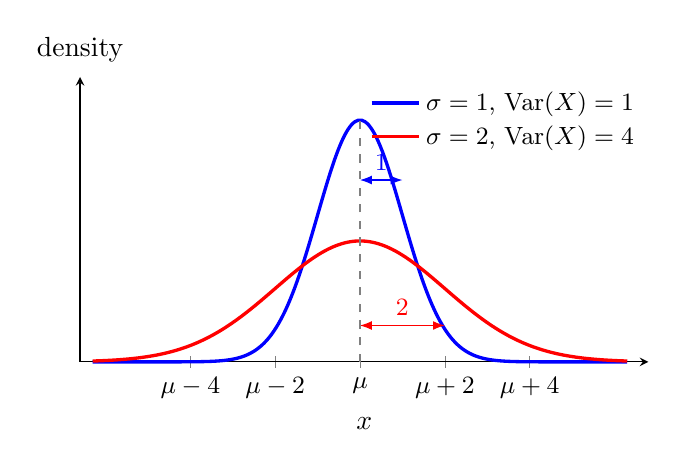
\begin{tikzpicture}
	\begin{axis}[
		axis lines=left, xmin=-6.6, xmax=6.8, ymin=0, ymax=0.47,
		xtick={-4,-2,0,2,4}, xticklabels={$\mu-4$,$\mu-2$,$\mu$,$\mu+2$,$\mu+4$}, tick label style={font=\small}, ytick=\empty,
		xlabel={$x$}, ylabel={density}, ylabel style={rotate=-90, anchor=south, at={(axis description cs:0,1.02)}},
		samples=160, smooth, width=8.8cm, height=5.2cm, clip=false,
		legend style={draw=none, fill=none, font=\small, at={(1.0,0.99)}, anchor=north east}, legend cell align=left
		]
		\addplot[blue, very thick, domain=-6.3:6.3] {exp(-x^2/2)/sqrt(2*pi)};
		\addlegendentry{$\sigma=1$, $\operatorname{Var}(X)=1$}
		\addplot[red, very thick, domain=-6.3:6.3] {exp(-x^2/8)/(2*sqrt(2*pi))};
		\addlegendentry{$\sigma=2$, $\operatorname{Var}(X)=4$}
		\draw[blue, {Latex[length=1.5mm]}-{Latex[length=1.5mm]}] (axis cs:0,0.3) -- (axis cs:1,0.3);
		\node[blue, font=\small, anchor=south] at (axis cs:0.5,0.3) {$1$};
		\draw[red, {Latex[length=1.5mm]}-{Latex[length=1.5mm]}] (axis cs:0,0.06) -- (axis cs:2,0.06);
		\node[red, font=\small, anchor=south] at (axis cs:1,0.06) {$2$};
		\draw[gray, dashed] (axis cs:0,0) -- (axis cs:0,0.399);
	\end{axis}
	
\end{tikzpicture}
\end{document}
